% \appendix
\renewcommand{\thechapter}{A}
\chapter{Appendix}

\definecolor{codegreen}{rgb}{0,0.6,0}
\definecolor{codegray}{rgb}{0.5,0.5,0.5}
\definecolor{codepurple}{rgb}{0.58,0,0.82}
\definecolor{backcolour}{rgb}{0.95,0.95,0.92}

\lstdefinestyle{mystyle}{
    backgroundcolor=\color{white},   
    commentstyle=\color{codegreen},
    keywordstyle=\color{magenta},
    numberstyle=\tiny\color{codegray},
    stringstyle=\color{codepurple},
    basicstyle=\ttfamily\footnotesize,
    breakatwhitespace=false,         
    breaklines=true,                 
    captionpos=b,                    
    keepspaces=true,                          
    showspaces=false,                
    showstringspaces=false,
    showtabs=false,                  
    tabsize=2
}

\lstset{style=mystyle}

\section*{GradCAM++ importance weights}\label{sec:grad-cam-plus-plus-weight-derivation}

Without the loss of generality, let us fix layer $K$ with the highest activation $A^k_{ij}$.
Since we utilize the GMP layer, all partial derivatives in \myref{Equation}{eq:grad-cam-pp-weights} will be zero, except for the one corresponding to the highest activation.
As a result, we get rid of both sums, and the importance weight becomes 
\begin{equation}
    i_{ck} = \alpha^{ck}_{ij} \relu(\frac{\partial Y^c}{\partial A^k_{ij}}).
\end{equation}
Authors already derived the activated score $Y^c = \exp(y^c)$ for us, and given the architecture of our model, the following set of equations holds:
\begin{equation}
\begin{aligned}
  \frac{\partial Y^c}{\partial A_{ij}^k}       &= \exp(y^c) \frac{\partial y^c}{\partial A_{ij}^k} &= \exp(y^c) w_{ck}     \\
  \frac{\partial^2 Y^c}{\partial (A_{ij}^k)^2} &= \exp(y^c) (\frac{\partial y^c}{\partial A_{ij}^k})^2 &= \exp(y^c) (w_{ck})^2 \\
  \frac{\partial^3 Y^c}{\partial (A_{ij}^k)^3} &= \exp(y^c) (\frac{\partial y^c}{\partial A_{ij}^k})^3 &= \exp(y^c) (w_{ck})^3.
\end{aligned}
\end{equation}

Plugging it all together, we get 
\begin{equation}
    \alpha_{ij}^{ck} = \frac{\exp(y^c) (w_{ck})^2}{2 \exp(y^c) (w_{ck})^2 + A^k_{ij} \exp(y^c) (w_{ck})^3} = \frac{1}{2 + A^k_{ij}w_{ck}}
\end{equation}
and subsequently
\begin{equation}
    i_{ck} = \frac{1}{2 + A^k_{ij}w_{ck}} \relu\bigr(\exp(y^c)w_{ck}\bigl).
\end{equation}

\section*{Convolutional Versus Pooling Layer for CAM-Based Methods}\label{sec:conv-vs-pool}

This thesis aims to find a performant explainability method that produces saliency maps similar to Occlusion.
While it seems natural to compute the saliency maps for the last convolutional layer, we decided to spend some time exploring our options.

The last convolutional layer produces $512$ activation maps, each comprising $32 \times 32$ activations.
When we upsample weighted activation map $A^k$ to the size of $512 \times 512$ pixels, each spatial activation corresponds to a $16 \times 16$ portion of the upsampled activation map.
When we use the last pooling layer instead, the dimensions flip, and individual elements of $16 \times 16$ pooled activation map will correspond to $32 \times 32$ pixels in the upsampled saliency map.
The production-grade setting for Occlusion uses a patch of $55 \times 55$ pixels, with $27$ pixels stride.
We believe that computing saliency maps for the pooled activations might closely resemble the ones produced by Occlusion.

While we verified that saliency maps for the pooling layer are visually more similar to Occlusion than saliency maps for the convolutional layer, such ``anecdotal'' conclusion is insufficient \cite{xai-anecdotal-evidence}.
By applying the pooling operation, we are condensing the original activation map to $25$ percent of its original size, and this may lead to a loss of information when reconstructing the saliency map, undermining faithfulness.
Thus, we conducted an additional experiment to compare both approaches using the faithfulness metric from \myref{Section}{sec:quant}.
The distribution of ROAD ratios is depicted in \myref{Figure}{fig:road-conv-vs-pool}, and a visual comparison of both approaches is presented in \myref{Figure}{fig:conv-vs-pool}

Based on the results, we decided to continue with saliency maps computed with respect to the pooling layer.
There is a negligible difference for CAM, and we posit the pooled saliency maps as more similar to Occlusion.
The same goes for HiResCAM; although the convolutional layer receives a much smaller spread, the saliency maps tend to be more scattered and blurred.
For GradCAM++, using the convolutional layer is not an option.
Because of the indirect proportion between activation strength and resulting importance weight, the less important regions are marked as more salient when computing the saliency map with respect to the last convolutional layer.
As we impute more of the area blurred based on the saliency strength, the actual important regions are taken into account, and the model's score for perturbed images starts to drop.
This is mostly tackled in the case of the pooling layer, as the more condensed activations seem to even out the indirect proportion. 
The difference for GradCAM++ regions imputed by the ROAD metric is shown in \myref{Figure}{fig:gradcampp-road-conv-vs-pool}

\begin{figure}
    \begin{center}
    \begin{minipage}{1\textwidth}
      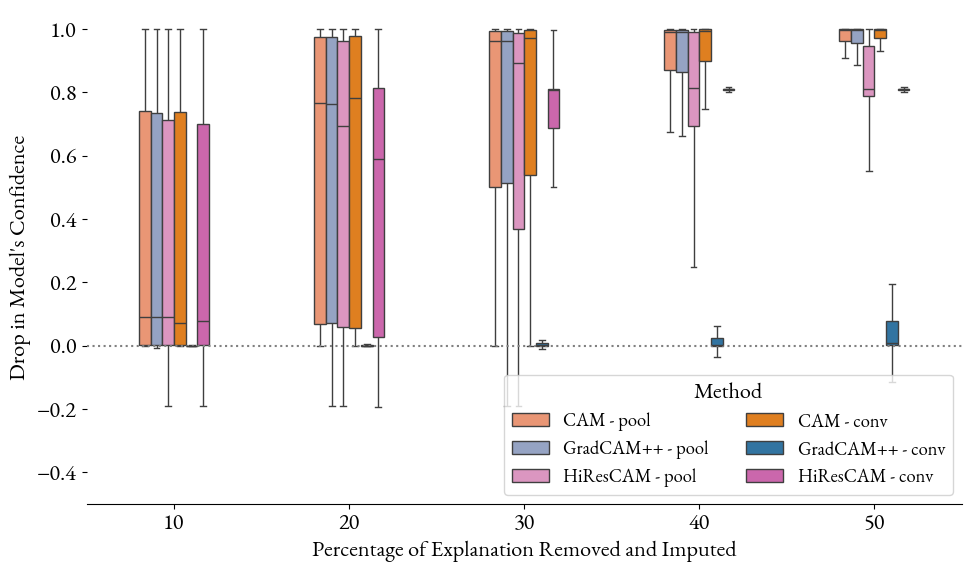
\includegraphics[width=\textwidth]{img/road-conv-vs-pool.png}
    \end{minipage}
    \caption{Comparison of ROAD ratios when attributing pooling versus convolutional layer. CAM scores are almost the same, with the convolutional layer saliency maps being slightly more faithful according to our metric. HiResCAM achieves a notably smaller spread when computing saliency maps with respect to the convolutional layer. However, the median is similar to its pooling layer counterpart. The biggest difference comes for GradCAM++. We believe it stems from our finding in \myref{Subsection}{sub:gradcampp}, where activation strength is indirectly proportional to the resulting importance weight.}
    \label{fig:road-conv-vs-pool}
    \end{center}
\end{figure}

\begin{figure}
    \begin{center}
    \begin{minipage}{0.5\textwidth}
      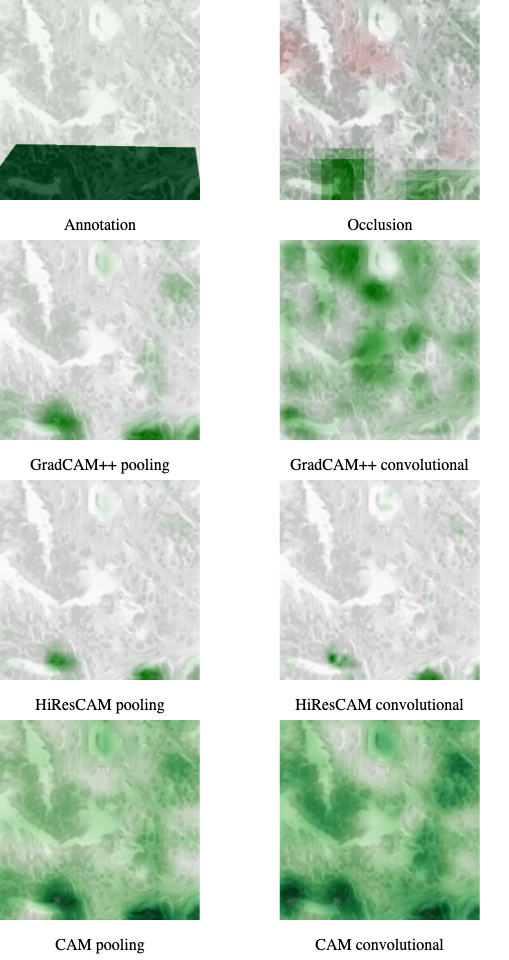
\includegraphics[width=\textwidth]{img/conv-vs-pool.png}
    \end{minipage}
    \caption{Visual comparison of saliency maps produced by CAM methods with respect to pooling and convolutional layer on a randomly selected tile. The underlying tile is presented in black and white to increase visual contrast. Notice that Occlusion falls within the annotation boundaries, except for the upper right corner. However, artifacts like this are removed using thresholding in the WSI browser. GradCAM++ completely differs when attributing the convolutional layer, focusing mostly on parts of the picture the Occlusion and annotation consider irrelevant. This changes once we compute the saliency maps with respect to the pooling layer. HiResCAM produces visually similar results, and despite producing similar results for this tile, the pooling saliency maps tend to cover larger and less scattered areas of the input tile. CAM is very liberal regarding the covered area, and the saliency maps are similar. However, the pooling one is easier to threshold because of the larger difference in saliency outside and within the annotated area.}
    \label{fig:conv-vs-pool}
    \end{center}
\end{figure}

\begin{figure}
    \begin{center}
    \begin{minipage}{0.75\textwidth}
      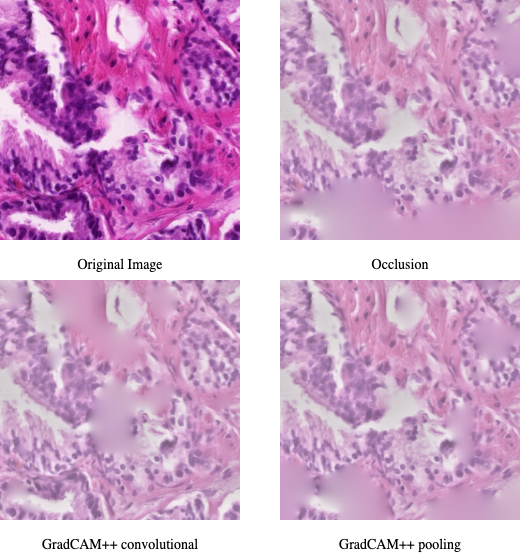
\includegraphics[width=\textwidth]{img/gradcampp-road-conv-vs-pool.png}
    \end{minipage}
    \caption{Visualization of different imputation results when we use the convolutional instead of the pooling layer. On the original tile, the model accurately reports $0.98$ confidence for the presence of cancer. Both Occlusion and GradCAM++ w.r.t pooling layer accurately point to the relevant locations in the bottom, and the confidence on perturbed tile drops to almost $0$. For GradCAM++ w.r.t. convolutional layer, the saliency map significantly differs from the other two, and the models' confidence stays the same. We used \texttt{pytorch-grad-cam}'s implementation of visualizing the perturbed input, hence the discoloration.}
    \label{fig:gradcampp-road-conv-vs-pool}
    \end{center}
\end{figure}